\documentclass[11pt,a4paper]{article}

\usepackage[a4paper,top=2.4cm,bottom=2.4cm,left=2.2cm,right=2.2cm]{geometry}
\usepackage{fontspec}
\usepackage[english,provide=*]{babel}
\babelprovide[import]{english}
\babelprovide[import]{spanish}
\babelfont{rm}{Noto Serif}
\babelfont{sf}{Noto Sans}
\babelfont{tt}{Noto Sans Mono}
\usepackage{amsmath,amssymb}
\usepackage{booktabs}
\usepackage{enumitem}
\usepackage{xcolor}
\usepackage{tikz}
\usetikzlibrary{arrows.meta,positioning,shapes.geometric,fit,backgrounds}
\usepackage[colorlinks=true,linkcolor=blue!60!black,citecolor=blue!60!black,urlcolor=blue!60!black]{hyperref}
\setlist[itemize]{label=--,leftmargin=*}
\setlist[enumerate]{leftmargin=*}
\emergencystretch=2em

\title{\textbf{ASTRA Production}\\[2mm]
\large An Autonomous Architecture for Scientific Theorem Reasoning and Validation}
\author{Nelson Bolívar\\\textit{Science-Stack Research Group}}
\date{Architecture version: September 2026}

\begin{document}
\maketitle

\begin{abstract}
ASTRA Production (\textit{Autonomous Symbolic Theorem Reasoning Architecture}) is a multi-agent research engine that turns scientific intuition into a falsifiable hypothesis, translates the hypothesis into an executable computational experiment, and critically analyzes the resulting evidence before accepting a conclusion. Its central design principle is the separation of language generation from evidence: language models propose, formalize, and analyze, while a symbolic or numerical computation oracle executes the validation program and returns reproducible evidence. The system supports isolated cycles and autonomous research campaigns, multiple model providers, local and remote mathematical engines, automatic code correction, human theorem approval, and persistent reports. A second design principle governs what happens when a cycle cannot conclude. Rather than forcing a verdict or exhausting its budget in repetition, ASTRA detects that a review loop has stopped making progress, declares an explicit undecidable outcome when the validator lacks inputs, and returns a structured request for the missing values instead of a silent failure. This document describes the currently implemented architecture, its guarantees, its limitations, and the present status of its evaluation.
\end{abstract}

\section{Motivation and epistemic principle}

Language models are useful for formulating hypotheses, connecting domains, and writing programs, but a plausible response is not a proof. ASTRA therefore adopts an explicit separation of responsibilities:

\begin{itemize}
  \item the \textbf{heuristic layer} proposes conjectures, generates code, and explains results;
  \item the \textbf{execution layer} computes with actual symbolic, numerical, or logical engines;
  \item the \textbf{control layer} preserves state, applies retries, guards verdicts, and requests human decisions;
  \item the \textbf{documentation layer} records code, output, analysis, providers, and research evolution.
\end{itemize}

ASTRA does not claim to automate mathematical truth. It turns AI-assisted reasoning into an inspectable process:
\[
\begin{aligned}
\text{intuition}&\longrightarrow\text{falsifiable hypothesis}
\longrightarrow\text{program}\\
&\longrightarrow\text{executed evidence}
\longrightarrow\text{reviewable verdict}.
\end{aligned}
\]

Model output never replaces execution. Conversely, successful execution is not sufficient by itself: the program must faithfully represent the claim and produce a signal that discriminates validation from refutation.

\section{Current architecture}

ASTRA runs as a local application with a browser interface. A Flask server exposes the interface and control API, while an asynchronous orchestrator maintains the state machine in the background. Agents communicate with LLM providers through a common client layer, and the oracle routes generated code to the appropriate computation engine. The browser interface, MCP server, and subprocess tool invoke the same canonical cycle; they do not maintain parallel scientific implementations.

\begin{figure}[htbp]
\centering
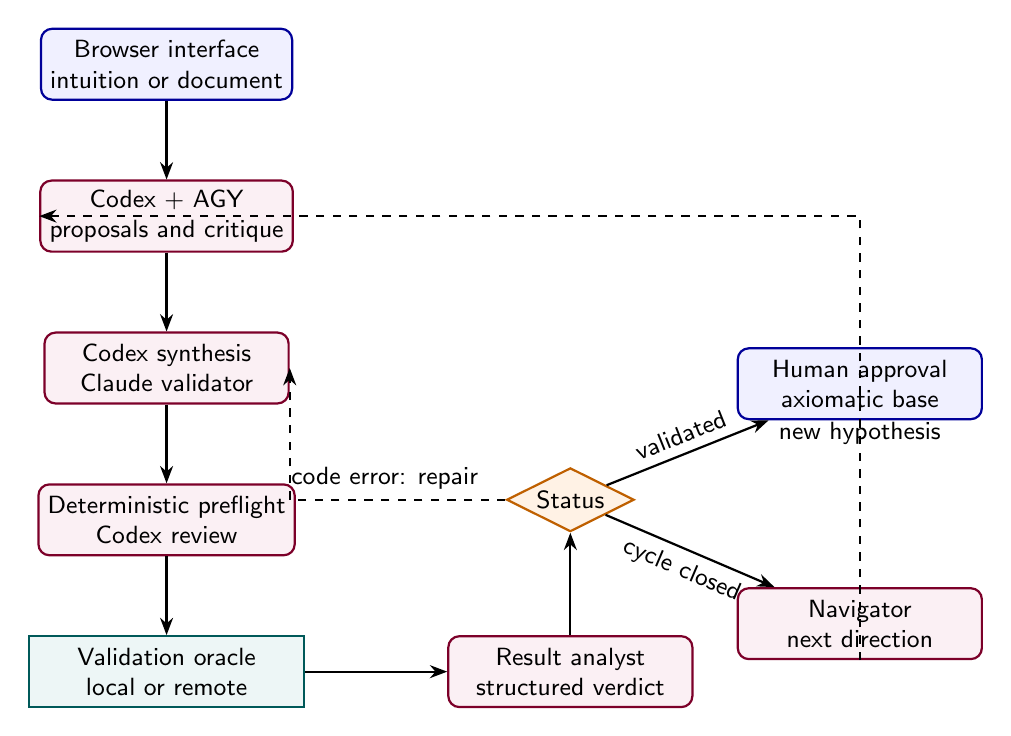
\begin{tikzpicture}[
  node distance=10mm and 9mm,
  font=\sffamily\small,
  ui/.style={rectangle,rounded corners,draw=blue!60!black,fill=blue!6,thick,align=center,minimum width=31mm,minimum height=9mm},
  agent/.style={rectangle,rounded corners,draw=purple!65!black,fill=purple!6,thick,align=center,minimum width=31mm,minimum height=9mm},
  oracle/.style={rectangle,draw=teal!70!black,fill=teal!7,thick,align=center,minimum width=35mm,minimum height=9mm},
  gate/.style={diamond,aspect=2,draw=orange!75!black,fill=orange!10,thick,align=center,inner sep=1.5pt},
  arr/.style={-{Stealth[length=2.2mm]},thick}
]
\node[ui] (input) {Browser interface\\intuition or document};
\node[agent,below=of input] (conj) {Codex + AGY\\proposals and critique};
\node[agent,below=of conj] (trans) {Codex synthesis\\Claude validator};
\node[agent,below=of trans] (review) {Deterministic preflight\\Codex review};
\node[oracle,below=of review] (exec) {Validation oracle\\local or remote};
\node[agent,right=18mm of exec] (analyst) {Result analyst\\structured verdict};
\node[gate,above=13mm of analyst] (status) {Status};
\node[ui,above right=8mm and 17mm of status] (human) {Human approval\\axiomatic base};
\node[agent,below right=9mm and 17mm of status] (nav) {Navigator\\next direction};

\draw[arr] (input)--(conj);
\draw[arr] (conj)--(trans);
\draw[arr] (trans)--(review);
\draw[arr] (review)--(exec);
\draw[arr] (exec)--(analyst);
\draw[arr] (analyst)--(status);
\draw[arr] (status)--node[above,sloped]{validated}(human);
\draw[arr] (status)--node[below,sloped]{cycle closed}(nav);
\draw[arr,dashed] (status.west) -| node[pos=.28,above]{code error: repair} (trans.east);
\draw[arr,dashed] (nav.south) |- node[pos=.28,below]{new hypothesis} (conj.west);
\end{tikzpicture}
\caption{Logical flow of ASTRA Production. The Navigator participates in Research Loop mode, while human approval protects admission of results to the axiomatic base.}
\label{fig:architecture}
\end{figure}

\subsection{Input and interface}

The user may enter a claim directly or upload PDF/TXT material. The application provides two operating modes:

\begin{itemize}
  \item \textbf{Single Cycle}: evaluates one concrete intuition through a complete pass.
  \item \textbf{Research Loop}: decomposes a macro-level question into a sequence of related conjectures and preserves alternative branches.
\end{itemize}

The interface displays status, the current conjecture, generated script, oracle output, axiomatic base, reports, and event log. It also lets the user stop execution, approve or reject results, and configure providers for each role. The cycle cache includes the shared objective, axiomatic base, reflective trajectory summary, distance from the last milestone, and non-secret model/control configuration. A repeated direction in a changed scientific context therefore cannot replay a stale navigation decision.

\subsection{Request structuring}

A raw request often carries several claims at once, or states an aim without a decidable criterion. An optional pre-cycle stage rewrites it into a bounded claim, an explicit hypothesis, a decisive test with its auxiliary checks, a proposed route, the inputs the test requires, and anything deliberately deferred. The cycle then works on the structured form while the original text is preserved alongside it, so the reader can always see what was asked and what was tested. The stage is opt-in because it costs one model call and a well-posed request does not need it.

Its practical value is the inputs list. A request that names the quantities a validator will need can be answered before the cycle starts, which is cheaper than discovering the gap after formalization.

\subsection{Conjecture agent}

Codex GPT-5.6 Sol and AGY receive the same final objective, current direction, and accumulated context. They propose in parallel, each adversarially critiques its rival proposal, and Codex synthesizes one falsifiable conjecture with variables, assumptions, domain, and success criterion. In iterative mode they also use established theorems and previous refutations to avoid reopening closed paths.

\subsection{Formal translator}

The translator converts the conjecture into a self-contained validation script. The program must compute a discriminating quantity: a symbolic residual, identity, initial-condition check, inequality, counterexample, tensor property, or numerical comparison with explicit tolerances. It may declare the engine through an \texttt{ASTRA\_ENGINE} header and suggest local or remote execution through \texttt{ASTRA\_ORACLE}.

The translator does not issue the scientific verdict. It constructs the experiment by which the claim can be decided.

\subsection{Deterministic preflight and independent review}

Before execution, deterministic checks detect patterns that could produce a false validation, import defects, and known operational failures. Codex then compares Claude's script with both the shared objective and the exact conjecture. When a defect is locally repairable, Claude receives bounded instructions and returns an exact-replacement patch. Codex does not become the validator author. Reviewer rejection or an inapplicable patch yields an abstention or tool error, never scientific evidence.

The loop is bounded in two independent ways. A revision cap limits how many times the validator may be patched or regenerated, and a wall-clock check stops a loop that would consume the cycle budget on repair alone. Neither bound diagnoses why a loop is failing, so a third mechanism does. Each rejection is classified by the defect it describes, reading the reviewer's prose rather than its instruction list, because the instructions enumerate the legs to preserve and therefore look alike on every round. The classifier recognises a small set of recurring defects, among them an assumed bound, an undecidable positivity claim, a link asserted only in a comment, a proxy substituted for the quantity of interest, a missing domain restriction, and sampling presented as proof.

The response escalates with the evidence. A defect seen once produces a directed correction naming it. The same defect class seen again is treated as a sign that patching will not converge, and the cycle spends one regeneration on a different strategy rather than another patch. If the class survives that too, the cycle stops cleanly and reports the defect class it could not clear. A stop of this kind is an abstention with a named cause, which is more useful than a budget exhausted in silence. The detector is on by default and can be disabled for controlled comparisons.

\subsection{Validation oracle}

The oracle executes the program and captures return code, standard output, errors, and engine metadata. Python provides the common foundation, with libraries including SymPy, Z3, NumPy, SciPy, mpmath, EinsteinPy, Pint, fluids, and QuTiP. ASTRA can also route jobs to SageMath, Maxima, or Cadabra when available. On Windows, \texttt{ASTRA\_WSL\_DISTRO} pins the intended WSL2 distribution so that execution does not silently move when the machine's default distribution changes. The production workstation uses Debian/WSL2 for SageMath, Maxima, Cadabra, and the local Lean/Mathlib environment.

Execution may be:

\begin{itemize}
  \item \textbf{local}, suitable for symbolic algebra and moderate computation;
  \item \textbf{remote}, through an SSH-connected Linux worker for heavy workloads, GPU use, or tools installed on the compute workstation.
\end{itemize}

The policy may be fixed by configuration or inferred from markers and script characteristics. A missing optional engine must cause an explicit failure rather than a fabricated validation.

\subsection{Analyst and verdict guard}

The analyst receives the conjecture and raw evidence. It returns a structured response with one of these states:

\begin{center}
\begin{tabular}{@{}ll@{}}
\toprule
State & Meaning \\
\midrule
\texttt{VALIDATED} & Computational evidence supports the stated hypothesis. \\
\texttt{REFUTED} & Execution finds a counterexample or contradicts the hypothesis. \\
\texttt{NON\_DECIDABLE} & The test cannot be instantiated because declared inputs are missing. \\
\texttt{CODE\_ERROR} & The program failed to execute the intended test correctly. \\
\texttt{API\_ERROR} & The LLM provider, network, or relevant quota failed. \\
\bottomrule
\end{tabular}
\end{center}

A sixth state, \texttt{WEAK\_PASS}, is not produced by the analyst but imposed on it. The verdict guard audits the validator's syntax tree and downgrades a pass that no reachable failure branch could have contradicted, which is the signature of a test that cannot fail. When independent analyses disagree, the most prudent reading wins under a fixed precedence, with refutation ahead of undecidability, undecidability ahead of code error, and any of them ahead of validation. A provider failure is handled separately, since it carries no scientific content at all.

When a \texttt{CODE\_ERROR} occurs, ASTRA requests corrected code and reruns validation up to the configured limit. The verdict guard restricts conclusions that are incompatible with execution evidence. This reduces, but does not eliminate, the risk that the analyst will turn a technical failure into a scientific claim.

\subsection{When the inputs are missing}

A validator that cannot be instantiated is not a refutation and not a bug, yet for most of ASTRA's history it was recorded as the latter. A test missing a boundary value, a material constant, or an ansatz would fail to run, be classified as a code error, and consume the full repair budget regenerating a program that was never the problem.

The undecidable outcome makes that case first class. The validator declares it explicitly, printing a verdict marker followed by one line per missing input and exiting with a reserved status. The declaration must come from the validator itself. An analyst may confirm an undecidable outcome only when the program declared one, so the state cannot be invented after the fact to excuse a failure. One retry is permitted if the analyst insists the program was merely broken. A second declaration, or a repair the author reports as impossible, closes the cycle.

\subsection{Asking instead of stopping}

Ending undecided is an honest outcome but a poor default, because the missing value is often one the researcher has. ASTRA has no channel of its own to the user, so the question travels in the result to whichever agent invoked the cycle. An undecidable result carries a request naming the missing inputs and three ways to answer, each with the exact re-invocation that implements it. The user may supply the values, may instruct the cycle to assume declared values and proceed, or may have the calling agent extract them from a file or an earlier result.

Assumption is deliberately constrained. A validator running under that policy must declare each assumed value on its own line, those declarations are attached to the result as conditions, and a run that assumed anything can never certify the whole objective. Its coverage stays partial and its status stays atomic. A validator that was granted the assume policy and declared nothing is treated as if it had assumed silently, which is the more dangerous case, and is flagged the same way. Answers reuse the conjecture already paid for through the cycle's own checkpoint, so responding to the question restarts at the validator rather than at the beginning.

\subsection{Human approval and axiomatic base}

A hypothesis marked as validated remains pending. Only after researcher approval is it added as an established theorem. Refutations and their reasons also enter the working context so that discarded paths are not silently repeated. This human gate recognizes that program correctness, physical assumptions, and the scope of a conclusion still require expert judgment.

\section{Autonomous research loop}

During a campaign, ASTRA maintains a \textit{Research Session} associated with a macro question. After each cycle, the Navigator assesses progress and proposes:

\begin{itemize}
  \item the next depth-first research direction;
  \item parallel branches worth preserving;
  \item whether a milestone requiring review has been reached;
  \item whether the macro question may be considered resolved.
\end{itemize}

If a conjecture is validated, the system may generalize it, explore its boundaries, or apply it to another regime. If it is refuted, the system seeks an alternative that avoids the specific cause of failure. The researcher may accept the proposal, redirect the investigation, or activate a saved branch. In autonomous mode ASTRA passes milestones without pausing until the Navigator declares resolution, the maximum runtime is reached, or the user stops the session.

This is a depth-first procedure with branch memory; it is neither an exhaustive search nor a guarantee that a resolution declaration is correct.

\section{Controlling ASTRA from an agent}

ASTRA is not limited to its browser interface. Its Model Context Protocol (MCP) server exposes the oracle as tools callable by Codex, Claude Code, Gemini, or another compatible client. The agent conversing with the researcher can therefore plan the test, write the validation program, request execution, and inspect evidence without manually moving results between applications.

The interface has grown to roughly twenty operations in six families:

\begin{center}
\small
\begin{tabular}{@{}lp{10.0cm}@{}}
\toprule
Family & Operations \\
\midrule
Deliberation & \texttt{astra\_cycle} runs conjecture, translation, review, oracle, and analysis as one pass. \texttt{astra\_cycle\_submit} does the same detached, for cycles longer than a client's tool wall. \\
Execution & \texttt{astra\_execute} runs an existing script on the local, remote, or automatic oracle. \\
Jobs & \texttt{astra\_submit} and \texttt{astra\_job} start and poll detached computation with incremental output. \\
Observation & \texttt{astra\_probe} reads a live cycle's phase and heartbeat without interrupting it. \texttt{astra\_telemetry} summarises the finished pool. \texttt{astra\_status}, \texttt{astra\_engines}, and \texttt{astra\_capacity} report worker reachability, available engines, and free cycle slots. \\
Campaigns & \texttt{astra\_campaign\_*} start, step, inspect, pause, and resume a multi-cycle programme. \\
Cluster & \texttt{astra\_cluster\_*} submit, poll, and cancel work on the compute workstation. \\
\bottomrule
\end{tabular}
\end{center}

A cycle invoked through this interface accepts the same request fields the structuring and input machinery described above expose, which is what lets an agent answer an undecidable result without reconstructing the original call.

The MCP server is registered by pointing the client to ASTRA's environment interpreter and \path{mcp_server/server.py}; a new agent session is then opened so that the tools are loaded. The researcher may ask, for example, ``construct an independent test of the Ricci scalar, run it with \texttt{astra\_execute}, and do not accept the result until the residuals have been inspected.'' Computations longer than a few minutes should use \texttt{astra\_submit} and be followed with \texttt{astra\_job}.

This mode makes the conversational agent the planning layer and ASTRA the traceable execution layer. The agent receives no additional authority: it must still expose code, assumptions, output, and the decision criterion.

\section{Extension through scientific engines and packages}

The oracle layer is extensible rather than a closed list. Any package available in the execution environment may participate in validation. In-house scientific packages include:

\begin{center}
\path{GR_python}\quad \path{pyWarpFactory}\quad \path{warp_bubble_optimization}.
\end{center}

Integration has a simple contract: the script must import the package, fix reproducible inputs, produce inspectable evidence, and end with an explicit verdict. The same package must be installed in the selected local or remote environment.

This mechanism allows ASTRA to reuse validated solvers, metrics, optimizers, energy-condition analyses, and test suites. Important conclusions should combine independent legs whenever possible---for example, a symbolic identity, fixed-seed numerical evaluations, and a known limiting case.

\subsection{Lean 4 and Mathlib}

Lean 4 is integrated as an optional engine through the marker \texttt{\# ASTRA\_ENGINE: lean}. The translator may generate a file importing Mathlib; ASTRA passes it either to a pinned native project, to the pinned Debian/WSL2 project, or to the configured ASTRUM formal route. The production local route fixes Lean 4.30.0 and the Mathlib commit beginning \texttt{c5ea00351c28}. Acceptance by the Lean kernel provides mechanical verification suitable for formal logic, discrete mathematics, algebra, and theorems that can be represented in the proof assistant's language.

Lean does not replace numerical physics calculations or prove that a formalization faithfully represents a physical system. Its guarantee applies to the formal statement and imported axioms. If the compiler rejects a proof, ASTRA classifies the event as a code error and may request a correction; rejection must never be turned into a refutation of the theorem.

\subsection{Wolfram Mathematica as a complementary oracle}

When the model has access to a Wolfram plugin or the \path{mathematica-agent-bridge} project, the agent can write and execute Wolfram Language directly. The local bridge connects external processes to a Mathematica kernel through a JSON queue and can operate on an open notebook or headlessly through \texttt{wolframscript}. Its actions include \texttt{evaluate-wl}, \texttt{simplify-symbolic}, \texttt{compare-expressions}, \texttt{commutator}, and \texttt{gr-curvature}, as well as reading, writing, and evaluating notebook cells.

Mathematica can act as a second independent validator: the agent runs a test through ASTRA and repeats the identity, tensor, or limit through the bridge. Agreement between independently implemented engines strengthens the evidence; disagreement triggers inspection of conventions, domains, and assumptions. The bridge evaluates code with the local user's privileges and should therefore be enabled only for trusted agents and command folders.

\section{Providers, engines, and deployment}

Roles may be reassigned for controlled ablations, but the compact production contract is explicit: Codex CLI with \texttt{gpt-5.6-sol} at \texttt{xhigh} effort proposes, synthesizes, reviews, and analyzes; AGY with \texttt{gemini-3.1-pro-high} at \texttt{high} effort is the primary co-proposer, critic, and navigator, with \texttt{gemini-3.7-flash-high} as the first configured fallback and \texttt{gemini-3.5-flash-high} as a legacy fallback; Claude Code with \texttt{claude-opus-4-8} writes and repairs code. The \texttt{scripts/audit\_architecture.py} command verifies this map, the binaries, epistemic gates, local scientific engines, and configured formal routes without reading or printing secrets. \texttt{ASTRA\_REQUIRED\_LOCAL\_ENGINES} makes missing production engines a blocking audit failure. The idempotent \path{scripts/bootstrap_wsl_scientific_stack.ps1} script recreates the pinned Debian stack. Other supported providers are reserved for controlled comparisons.

Providers are reached through their subscription command line clients rather than metered APIs, so the operating constraint is a per-model usage window rather than a per-token price. Each role therefore carries an ordered ladder of models. A quota failure descends the ladder and the result records which rung answered, while a quality failure climbs it, promoting the author to a stronger model exactly when the deterministic guard has demonstrated that the cheaper one was insufficient. A trial of an additional provider runs through the same client layer inside WSL and is treated as one more configurable role.

Configuration that could change a scientific result is stamped on every cycle. The architecture manifest records the role map, the effective models, the epistemic gates, and the required local engines, and it participates in the cycle cache key together with a schema version. Changing a control therefore invalidates cached cycles rather than silently reusing results produced under different rules.

The desktop installation creates a Python environment and launches the interface at \url{http://127.0.0.1:5050}. Credentials and oracle parameters remain in local configuration and must not be committed to the repository. ASTRA stores sessions and reports in the application's workspace.

\section{Persistence, traceability, and calibration}

Each cycle produces HTML and Markdown reports containing the intuition, conjecture, script, execution result, analysis, and selected providers. Investigations can be saved, reloaded, and reviewed through history. The benchmark suite covers general relativity, ordinary differential equations, fluid mechanics, logic, quantum systems, and symbolic computation.

Benchmarks serve two purposes: they verify that the engines remain operational and compare how well different providers construct discriminating tests. They do not replace scientific validation of a new problem, but they expose infrastructure regressions and systematic biases.

\section{Observability and execution hygiene}

A cycle that takes twenty minutes is normal, and for most of ASTRA's history it was also opaque. Three mechanisms now make a run inspectable while it happens and auditable afterwards.

Every cycle writes a heartbeat naming its current phase, its elapsed time per completed phase, and the checkpoint it belongs to. A reader process can therefore report progress without touching the cycle. On Windows each cycle also opens its own console showing the instruction, the phase, the review round, a progress bar, and an estimated finish time computed from the medians of recent finished cycles. The window is launched through a detached trampoline so that killing a timed out cycle does not also destroy the only account of what it was doing. Observability that dies with the process it observes is worth little precisely when it is needed.

Test runs are kept out of the production record. The pools that telemetry reads are the finished checkpoints and the live heartbeats, and a suite that exercises real cycles used to write into both, which distorted every duration and outcome count. A workspace root override redirects all cycle artefacts, and the test session sets it to a temporary directory. Without the variable the paths are byte for byte what they always were, so production behaviour is unchanged.

The system is also expected to fail intelligibly in hostile contexts. When ASTRA is driven from a sandboxed session whose access token cannot write to its own workspace, the phase now stops immediately with an explicit permissions error naming the directory and the two ways out. It previously hung, because the platform reports a directory as writable from its access list alone without consulting a restricted token, and the standard temporary directory routine trusts that report and retries. For the same reason the installation audit distinguishes an engine that is absent from an engine that is merely unreachable from the current context, since telling a user to reinstall a working tool is worse than telling them nothing.

\section{Guarantees and limitations}

ASTRA improves reproducibility because it preserves and executes the program, but it does not automatically turn a computational check into a universal proof. Several obligations remain:

\begin{itemize}
  \item verify that the formal conjecture matches the original question;
  \item inspect whether the code tests a weakened or circular version of the claim;
  \item distinguish numerical evidence, symbolic identity, and logical proof;
  \item state domains, units, boundary conditions, and tolerances;
  \item repeat results that depend on precision, grid, or platform;
  \item subject consequential conclusions to independent human review.
\end{itemize}

The states added since July carry their own caveats, and they are narrower than their names suggest:

\begin{itemize}
  \item \texttt{NON\_DECIDABLE} records that this validator, as written, could not be instantiated with the inputs available. It is a statement about one program and one set of inputs, never a claim that the question is undecidable in principle.
  \item A verdict produced under the assume policy is conditional on values the model chose. It is evidence about a parameterised family, and the assumed values must be read together with it.
  \item A stop attributed to a repeated defect class bounds cost. It does not establish that the reviewer's objection was correct, only that patching stopped converging.
  \item The defect classifier reads prose written by a model and can misclassify. It is a scheduling heuristic for how to spend the remaining budget, not part of the evidence chain.
\end{itemize}

Thus, \texttt{VALIDATED} means ``validated by the oracle under the recorded program and assumptions,'' not ``absolute mathematical truth.'' ASTRA's strength lies in making the evidence chain visible and repeatable.

\section{Evaluation status}

This document describes an architecture. It does not yet report a measured advantage, and the distinction matters enough to state plainly.

What has been executed is a set of integration pilots, one case per external corpus, run on 24 July 2026 against SciCode, a FrontierScience olympiad problem, a miniF2F validation item, and an AInsteinBench repository task. They establish that the pipeline runs end to end on public material and that the reviewer and repair loop behave as designed on those cases. They are not leaderboard results, the raw reports are kept outside version control, and no claim of comparative performance rests on them.

A defensible comparison requires the complete official split of each benchmark, fixed prompts and budgets, declared retries, recorded evaluator versions, failures counted in the denominator, confidence intervals, and the native metric of each corpus, reported with wall time and model call counts.

The measurement that would most directly test this architecture is narrower than that and is the next planned experiment. The central design claim is that separating the author of a validator from its reviewer, across different model providers, catches defects that a single model reviewing its own work does not. That claim is testable by ablation at equal budget, comparing the production configuration against one in which the authoring model also reviews, and against one with no independent review at all, scoring how many defective validators reach the oracle in each arm. Until that experiment is run and its logs deposited, the argument for the architecture presented here is one of construction and traceability, not of demonstrated accuracy.

\section{Conclusion}

ASTRA Production has evolved from a fixed processing scheme into a configurable, iterative, multi-agent research architecture. Formulation, translation, execution, analysis, navigation, and approval are distinct responsibilities. The work since July has been less about adding capability than about bounding failure, so that a cycle which cannot conclude says which input it lacks, which defect it could not clear, or which permission it was denied, instead of consuming its budget in silence. The oracle provides a reference external to model discourse; reports preserve traceability; and the human gate prevents autonomy from being mistaken for scientific authority. The result is a platform for conducting research with language models without silently delegating to them the final criterion of truth.

\end{document}
